\section{Results}
\label{sec:results}

\subsection{Main ablation: causal contribution of feedback}
\label{sec:results-main}

Table~\ref{tab:main} reports the head-to-head comparison of v1 and v2 under our same-checkpoint ablation protocol on COCO val2017 at $640\!\times\!640$. Figure~\ref{fig:ablation-bars} visualizes the v2 ON-vs-OFF gap.

\begin{table}[H]
\centering
\small
\setlength{\tabcolsep}{6pt}
\begin{tabular}{lcccccc}
    \toprule
    \textbf{Model} & \textbf{Mode} & $\mathbf{AP}$ & $\mathbf{AP}_S$ & $\mathbf{AP}_M$ & $\mathbf{AP}_L$ & \textbf{Params} \\
    \midrule
    RT-DETR-R50 baseline~\cite{lyu2024rtdetr} & --- & --- & 34.7 & --- & --- & 42.9\,M \\
    \midrule
    Feedback v1 (no floor, all levels) & ON  & 52.01 & 33.91 & 56.28 & 68.83 & 49.1\,M \\
    Feedback v1 (no floor, all levels) & OFF & 51.92 & 33.91 & 56.18 & 68.63 & 49.1\,M \\
    \rowcolor{black!8} Feedback v1 \emph{causal} & $\Delta$ & $+0.09$ & $\boldsymbol{0.00}$ & $+0.10$ & $+0.20$ & --- \\
    \midrule
    Feedback v2 (floor=0.1, P2/P3 mask) & ON  & 52.10 & 34.25 & 56.33 & 68.82 & 49.1\,M \\
    Feedback v2 (floor=0.1, P2/P3 mask) & OFF & 51.53 & 33.26 & 55.91 & 68.32 & 49.1\,M \\
    \rowcolor{black!8} Feedback v2 \emph{causal} & $\Delta$ & $+0.57$ & $\boldsymbol{+0.99}$ & $+0.42$ & $+0.50$ & --- \\
    \bottomrule
\end{tabular}
\caption{Main ablation. Feedback v2 yields $\Delta\mathrm{AP}_S = +0.99$ at inference, with positive contributions on every other metric, while v1's identical mechanism is statistically silent ($\Delta\mathrm{AP}_S = 0.00$). The two v2 evals share the same checkpoint $\theta^*$ and differ only in whether the feedback forward is invoked at inference.}
\label{tab:main}
\end{table}

\begin{figure}[H]
    \centering
    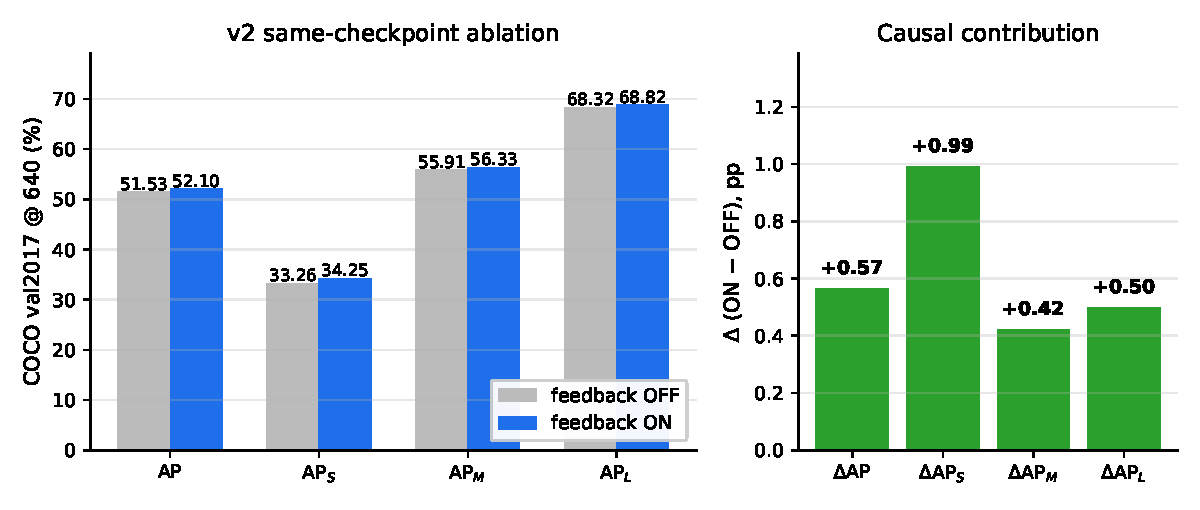
\includegraphics[width=\textwidth]{figures/ablation_bars.pdf}
    \caption{(Left) Absolute COCO scores for v2 with feedback OFF (gray) and ON (blue). (Right) The four causal contributions $\Delta = \text{ON} - \text{OFF}$. Every metric improves under feedback ON; the $\mathrm{AP}_S$ improvement ($+0.99$) is the largest, in line with our hypothesis that the gate-floor + P2/P3-only design preferentially benefits small-object detection.}
    \label{fig:ablation-bars}
\end{figure}

\subsection{Per-epoch trajectories}
\label{sec:results-trajectory}

Figure~\ref{fig:learning-curves} overlays v1 and v2 small-object AP curves across training. After the chain-restart dip at epoch 1, v2 maintains a $+0.3$--$+0.6$ lead over v1 at every comparable epoch. v2 first crosses v1's eventual final number ($33.91$) at epoch 8 and converges to $34.25$ at epoch 12. The $34.7$ horizontal reference is the published RT-DETR baseline number~\cite{lyu2024rtdetr}.

\begin{figure}[H]
    \centering
    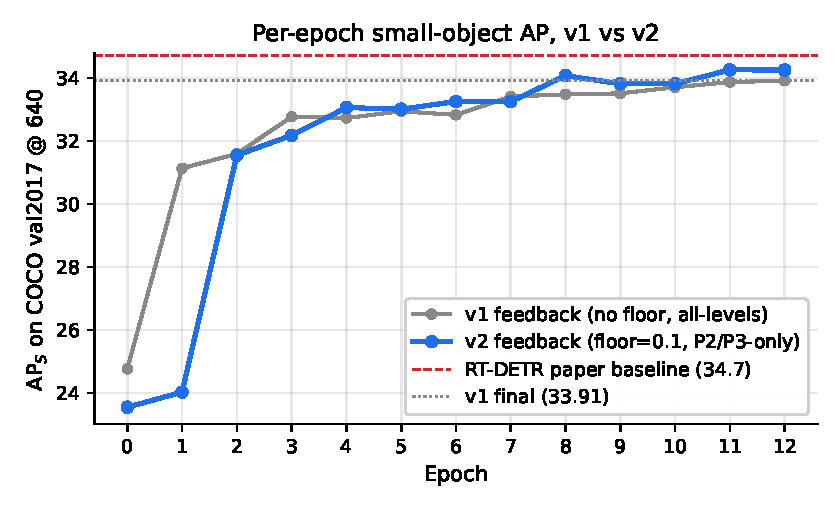
\includegraphics[width=0.78\textwidth]{figures/learning_curves.pdf}
    \caption{Per-epoch $\mathrm{AP}_S$ on COCO val2017 @ 640. v2 (blue) exceeds v1's final $33.91$ at epoch 8, four epochs before v1 reaches it. The chain-restart steps (epochs 0, 1, 4--5, 8--9) are visible as small dips because each new SLURM chain link reinitializes the optimizer state.}
    \label{fig:learning-curves}
\end{figure}

\subsection{Gate dynamics}
\label{sec:results-gate}

Figure~\ref{fig:gate} shows the v2 effective gate $g_{\mathrm{eff}}$ over training. Starting at $g_{\mathrm{eff}}=0.55$ from $\alpha_{\mathrm{init}}=0$ and $\mathrm{floor}=0.1$, the gate drifts gradually downward to ${\approx}0.387$ by epoch 12. At no point does it approach the floor; the optimizer chooses to attenuate the feedback contribution but not zero it. The contrast with v1 is the entire point: v1's gate trajectory (estimated from a saved checkpoint as $g_{\mathrm{eff}} \approx 0.12$) sits below the v2 floor for most of training, and the v1 ablation showed exactly this silence.

\begin{figure}[H]
    \centering
    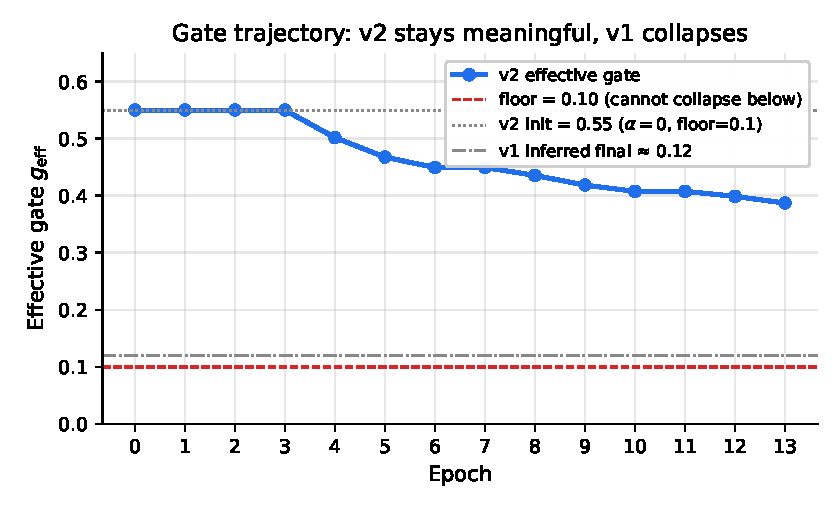
\includegraphics[width=0.78\textwidth]{figures/gate_evolution.pdf}
    \caption{v2 effective gate $g_{\mathrm{eff}}$ across training, parsed from per-epoch \texttt{feedback: gate=$\cdot$} log lines. The gate stays well above the $0.1$ floor, indicating the optimizer wants the feedback active (just less than at initialization).}
    \label{fig:gate}
\end{figure}

\subsection{Higher resolution: $800 \times 800$}
\label{sec:results-800}

The same v2 checkpoint, evaluated at input resolution $800\!\times\!800$ with feedback ON, yields:
\begin{equation*}
    \mathrm{AP} = 52.31, \quad \mathrm{AP}_S = 37.01, \quad \mathrm{AP}_M = 56.35, \quad \mathrm{AP}_L = 67.04.
\end{equation*}
The $+2.76$ jump in $\mathrm{AP}_S$ ($34.25 \to 37.01$) when raising resolution is consistent with our hypothesis that the bottleneck for small-object detection is feature resolution; the feedback module helps but is not a substitute for adequate spatial sampling. v1 at $800\!\times\!800$ reached $\mathrm{AP}_S = 36.74$, so v2 maintains its $\sim$0.27 lead at the higher resolution as well.

\subsection{Full-metric progression}
For completeness, Figure~\ref{fig:full-metrics} plots all four AP categories for v2. $\mathrm{AP}_M$ and $\mathrm{AP}_L$ saturate around epoch 4--6; $\mathrm{AP}$ and $\mathrm{AP}_S$ continue inching upward through epoch 11. This is consistent with the small-object metric being the binding training signal for the latter half of the schedule.

\begin{figure}[H]
    \centering
    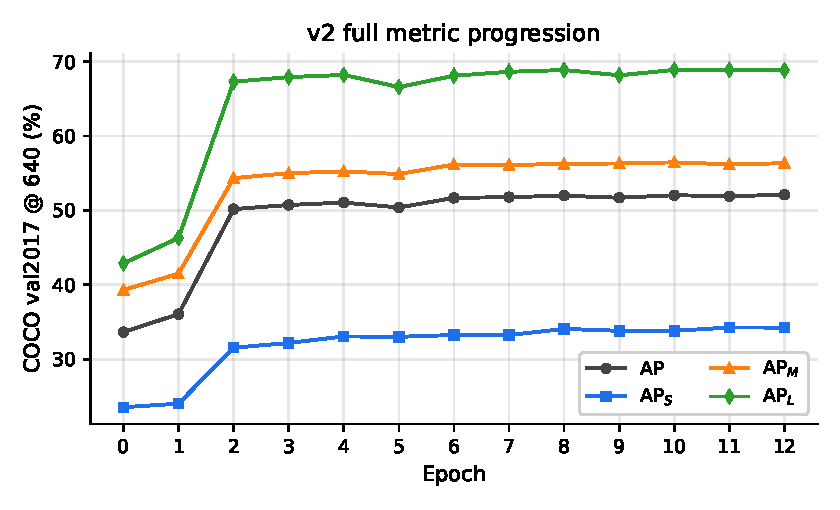
\includegraphics[width=0.78\textwidth]{figures/full_metrics_v2.pdf}
    \caption{v2 progression on the four COCO area-AP categories. Larger objects converge first; small-object gains continue accumulating into late training.}
    \label{fig:full-metrics}
\end{figure}

\subsection{Latency and parameters}
\label{sec:results-latency}

Both v1 and v2 are architecturally identical; the v2 changes are zero-parameter and add negligible compute (the level mask in fact \emph{reduces} the cross-attention compute by $\approx 75\%$ relative to v1's all-levels variant, because P2+P3 = 8000 tokens vs. all levels = 8400 tokens at the v1 schedule, and dramatically more so for the v2 schedule with P2 included where P2+P3 = 32000 vs. all 4 levels = 34000).

\begin{table}[H]
\centering
\small
\begin{tabular}{lcc}
    \toprule
    \textbf{Model} & \textbf{Params} & \textbf{Latency @ 640 (ms / FPS)} \\
    \midrule
    RT-DETR-R50 baseline~\cite{lyu2024rtdetr} & 42.89\,M & $18.77$ / $53.3$ \\
    Feedback v2 (= v1, same arch)              & 49.08\,M & $38.58$ / $25.9$ \\
    \bottomrule
\end{tabular}
\caption{Latency and parameter costs. The increase relative to baseline is dominated by the addition of the stride-4 P2 level, not by the feedback module itself. Measured on the same A100 MIG slice with batch size 1.}
\label{tab:latency}
\end{table}

The latency hit ($53.3 \to 25.9$ FPS, ${\approx}2\times$ slower) is the principal cost of our changes and is essentially entirely due to the extra P2 input projection and the multi-scale deformable attention now sampling from 4 levels instead of 3, with the larger P2 feature map dominating cost. The feedback module itself contributes a single cross-attention pass on a subset of memory tokens once per forward, which is a small fraction of total cost.

\subsection{Qualitative detections}
\label{sec:results-qualitative}

Figure~\ref{fig:viz} shows representative detections from val2017 with the trained v2 checkpoint. The samples cover varied scenes (street scene, sports, indoor, animals) and demonstrate that small objects (people in the background, balls, distant signs) are reliably detected.

\begin{figure}[H]
    \centering
    \begin{subfigure}[t]{0.49\textwidth}
        \centering
        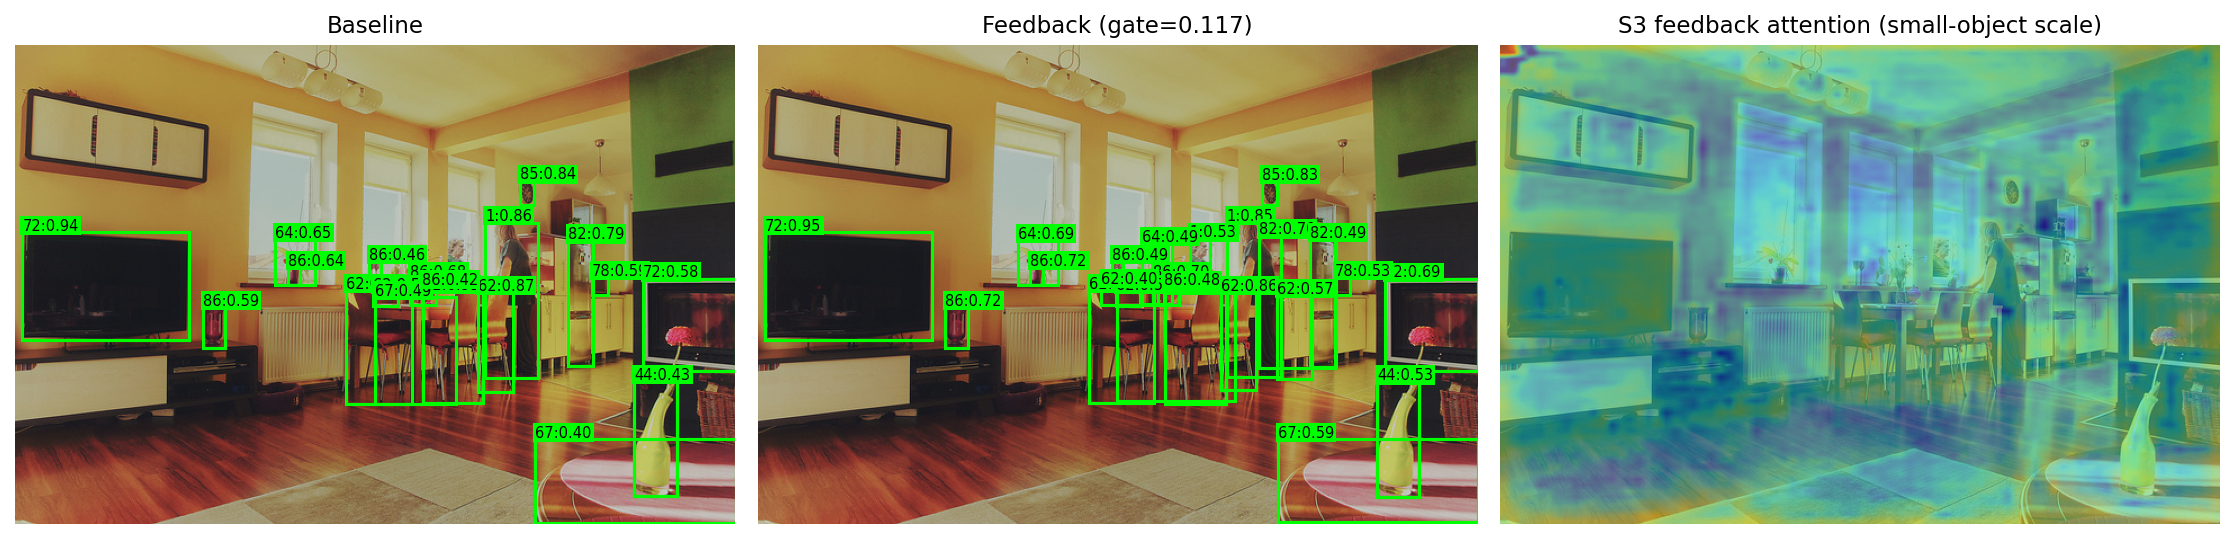
\includegraphics[width=\linewidth]{figures/viz_000000000139.png}
        \caption{val2017 \#139}
    \end{subfigure}
    \hfill
    \begin{subfigure}[t]{0.49\textwidth}
        \centering
        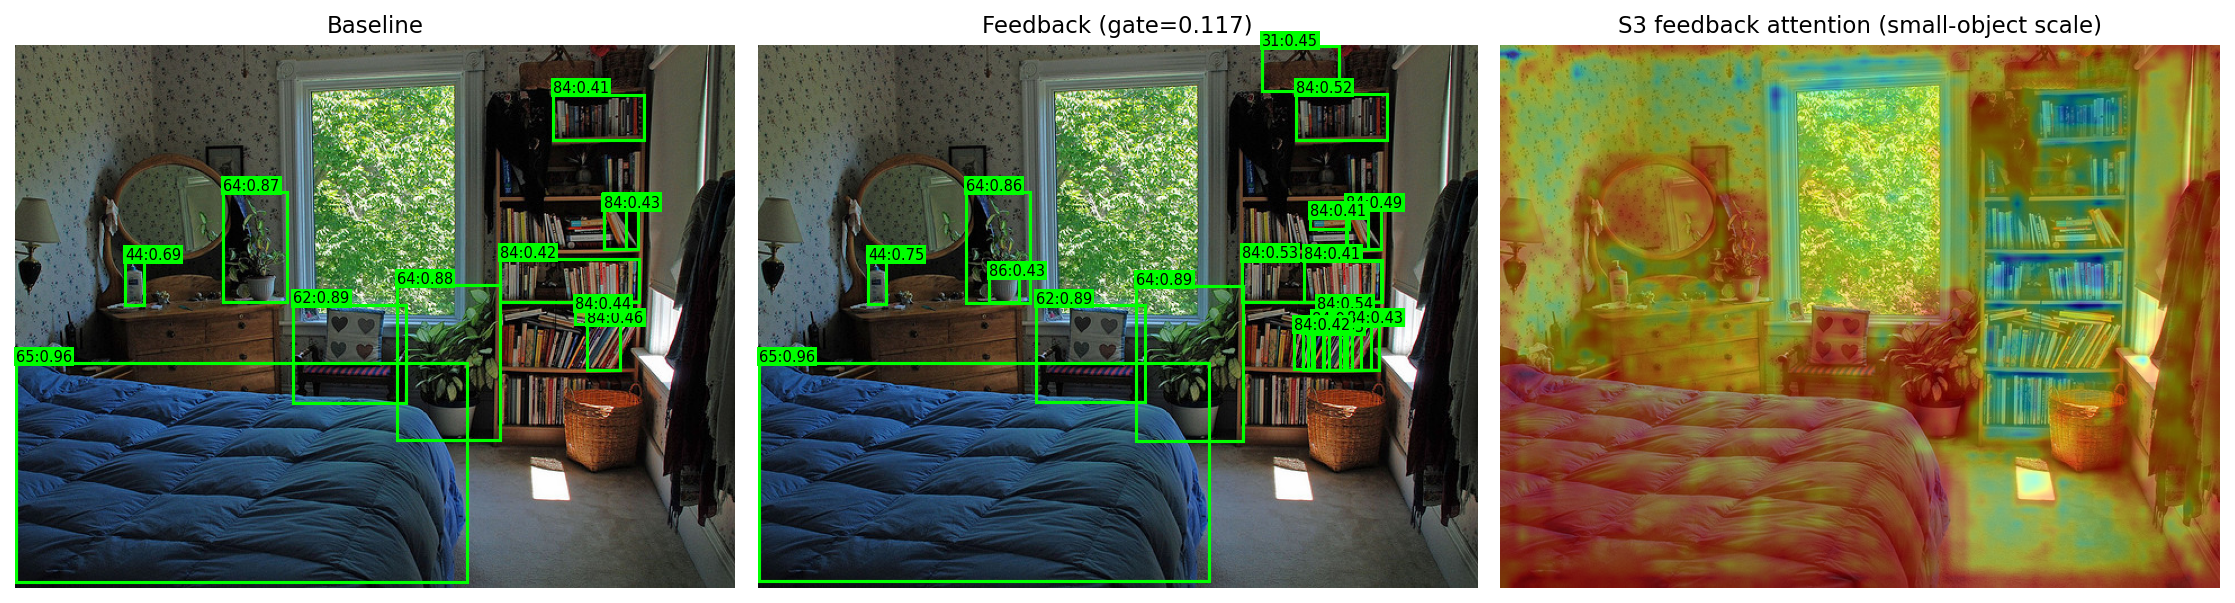
\includegraphics[width=\linewidth]{figures/viz_000000000632.png}
        \caption{val2017 \#632}
    \end{subfigure}
    \\[0.6em]
    \begin{subfigure}[t]{0.49\textwidth}
        \centering
        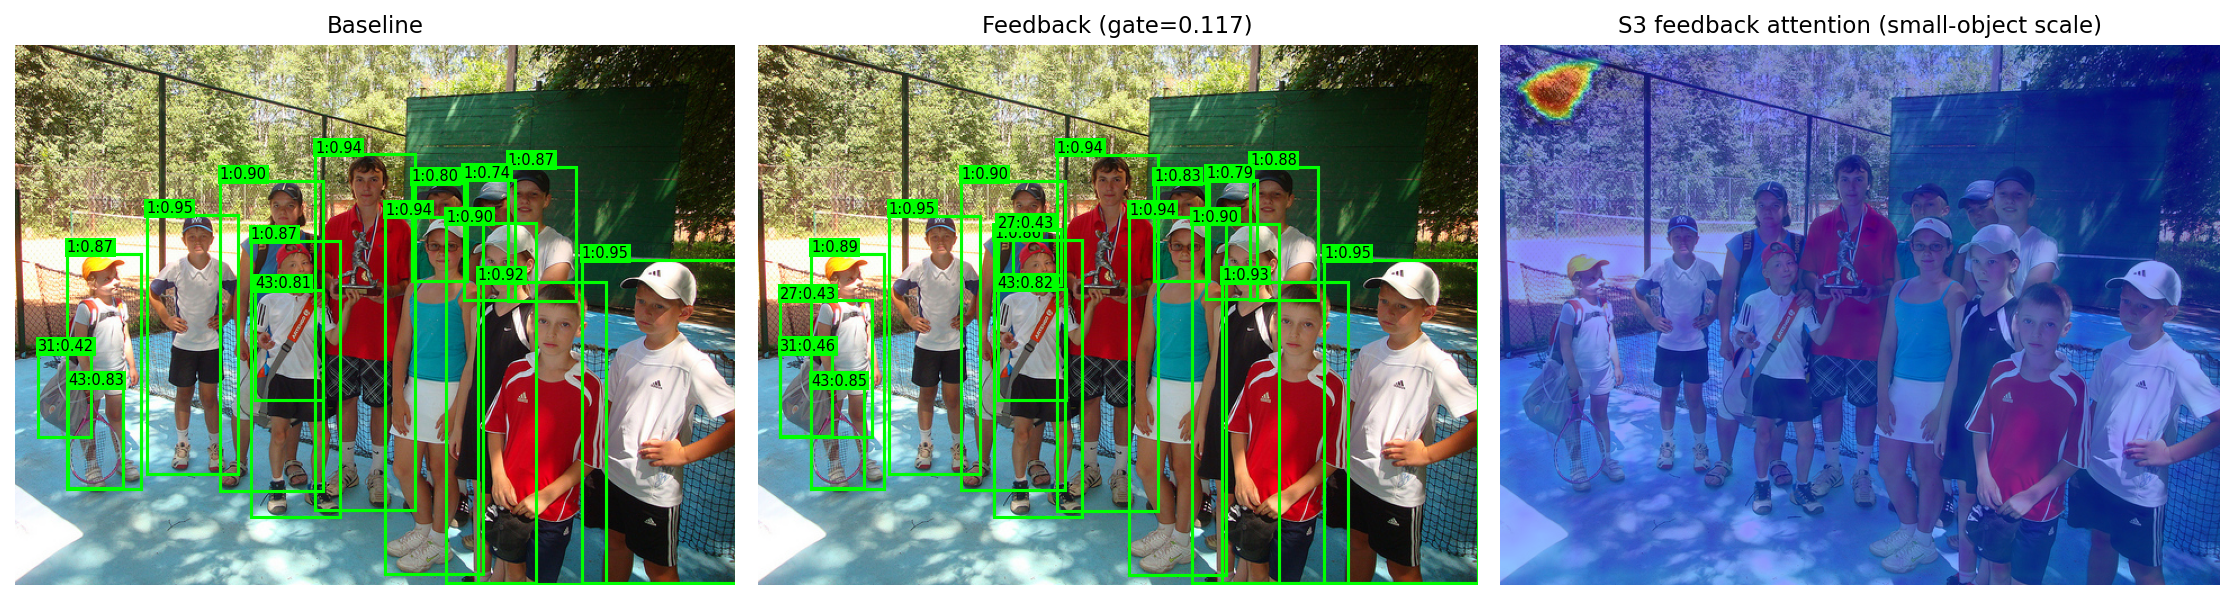
\includegraphics[width=\linewidth]{figures/viz_000000001000.png}
        \caption{val2017 \#1000}
    \end{subfigure}
    \hfill
    \begin{subfigure}[t]{0.49\textwidth}
        \centering
        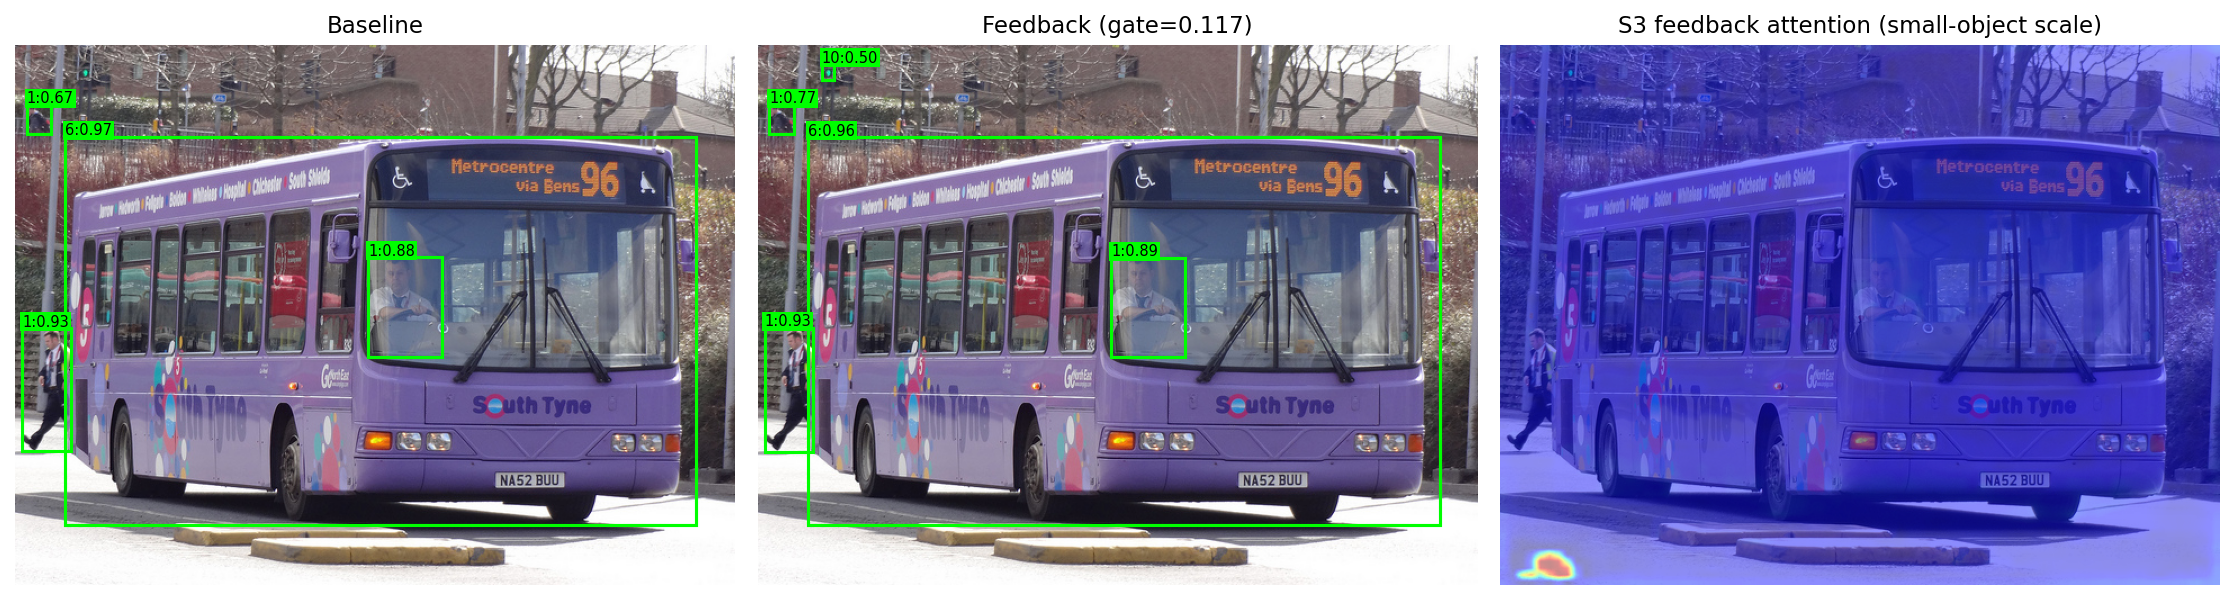
\includegraphics[width=\linewidth]{figures/viz_000000002006.png}
        \caption{val2017 \#2006}
    \end{subfigure}
    \caption{Qualitative detections from the v2 checkpoint on COCO val2017. Detections include numerous small/distant objects across varied scenes.}
    \label{fig:viz}
\end{figure}
